\RequirePackage{luatex85}
\documentclass[amsmath]{article}
\usepackage{amsmath}
\usepackage{amssymb}
\usepackage{geometry,contour}
\usepackage{tikz}
\usetikzlibrary{positioning}
\usetikzlibrary{decorations.text}
\usetikzlibrary{decorations.pathmorphing}
\usetikzlibrary{decorations.text}
\usetikzlibrary{decorations.pathmorphing}
\definecolor{darkolivegreen}{rgb}{0.3, 0.5, 0.2}
\geometry{legalpaper, landscape, margin=0.0in}
\paperheight 1.8in
\paperwidth 5.7in




\begin{document}
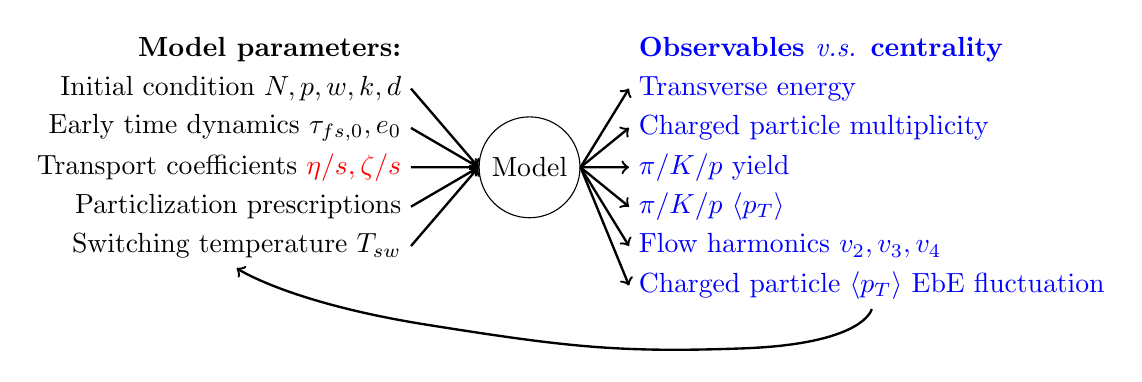
\begin{tikzpicture}
\node(a)[align=right] at (0,0) {\bf Model parameters:};
\node(b)[below=of a.east,anchor=east, yshift=.5cm] {Initial condition $N,p, w, k, d$};
\node(c)[below=of b.east,anchor=east, yshift=.5cm] {Early time dynamics $\tau_{fs,0}, e_0$};
\node(d)[below=of c.east,anchor=east, yshift=.5cm] {Transport coefficients \color{red}$\eta/s, \zeta/s$};
\node(e)[below=of d.east,anchor=east, yshift=.5cm] {Particlization prescriptions};
\node(f)[below=of e.east,anchor=east, yshift=.5cm] {Switching temperature $T_{sw}$};
\node(A) at (7,0) {\color{blue} \bf Observables  {\it v.s.} centrality};
\node(B) [below=of A.west,anchor=west, yshift=.5cm]{\color{blue} Transverse energy};
\node(C) [below=of B.west,anchor=west, yshift=.5cm]{ \color{blue} Charged particle multiplicity};
\node(D) [below=of C.west,anchor=west, yshift=.5cm] {\color{blue} $\pi$/$K$/$p$ yield};
\node(E) [below=of D.west,anchor=west, yshift=.5cm] {\color{blue} $\pi$/$K$/$p$ $\langle p_T \rangle$};
\node(F) [below=of E.west,anchor=west, yshift=.5cm] {\color{blue} Flow harmonics $v_2, v_3, v_4$};
\node(G) [below=of F.west,anchor=west, yshift=.5cm] {\color{blue} Charged particle $\langle p_T \rangle$ EbE fluctuation};

\node(H)[draw, circle] at(3.3,-1.5){Model};

\draw[->, color=black,line width=.3mm] (b.east)--(H.west);
\draw[->, color=black,line width=.3mm] (c.east)--(H.west);
\draw[->, color=black,line width=.3mm] (d.east)--(H.west);
\draw[->, color=black,line width=.3mm] (e.east)--(H.west);
\draw[->, color=black,line width=.3mm] (f.east)--(H.west);

\draw[->, color=black,line width=.3mm] (H.east)--(B.west);
\draw[->, color=black,line width=.3mm] (H.east)--(C.west);
\draw[->, color=black,line width=.3mm] (H.east)--(D.west);
\draw[->, color=black,line width=.3mm] (H.east)--(E.west);
\draw[->, color=black,line width=.3mm] (H.east)--(F.west);
\draw[->, color=black,line width=.3mm] (H.east)--(G.west);

\draw [->, color=black,line width=.3mm] plot [smooth, tension=1] coordinates { (G.south) (6,-3.8)(2,-3.5)(f.south)};
\end{tikzpicture}
\end{document}




